\title{Retrieval and analysis of Eurostat open data with the \pkg{eurostat} package}
\author{Leo Lahti, Janne Huovari, Markus Kainu, Przemyslaw Biecek}

\maketitle

%An abstract of less than 150 words.
\abstract{The increasing availability of open statistical data resources is
providing novel opportunities for research and citizen
science. Efficient algorithmic tools are needed to realize the full
potential of the new information resources. We introduce
the \CRANpkg{eurostat} R package that provides a collection of custom
tools for Eurostat open data, including functions to query, download,
manipulate, and visualize these data sets in a smooth, automated and
reproducible manner. The online documentation provides detailed
examples on the retrieval and analysis of these spatio-temporal data
sets. The \CRANpkg{eurostat} R package provides remarkable
improvements over the previously available tools, and has been
extensively tested by an active user community. This contributes to
the growing ecosystem of R packages dedicated to reproducible research
in computational social science and digital humanities.}


\section{Introduction}

Eurostat, the statistical
office of the European Union, provides a rich collection of data
through its open data service\footnote{\url{http://ec.europa.eu/eurostat/data/database}}, which includes thousands of data sets
on European demography, economics, health, infrastructure, traffic and
other topics. The statistics are often available with great
geographical resolution and include time series spanning over several
years or decades.

Availability of algorithmic tools to access and analyse open data
collections can greatly benefit reproducible
research \citep{Gandrud13, Boettiger2015}, as complete analytical
workflows spanning from raw data to final publications can be made
fully replicable and transparent. Dedicated software packages help to
simplify, standardize, and automate analysis workflows, greatly
facilitating reproducibility, code sharing, and efficient data
analytics. The algorithms need to be customized to specific data
sources to accommodate variations in raw data formats, access details,
and typical use cases so that the end users can avoid repetitive
programming tasks and save time. A number of packages for governmental
and other sources have been designed to meet these demands, including
packages for the Food and Agricultural Organization (FAO) of the
United Nations (\CRANpkg{FAOSTAT}; \cite{FAOSTAT}), World Bank
(\CRANpkg{WDI}; \cite{WDI}), national statistics authorities
(\CRANpkg{pxweb}; \cite{pxweb}), Open Street Map
(\CRANpkg{osmar}; \cite{osmar}) and many other sources.

A dedicated R package for the Eurostat open data has been
missing. The \CRANpkg{eurostat} R package fills this gap. It combines the relevant parts from our earlier \CRANpkg{statfi} \citep{statfi}
and \CRANpkg{smarterpoland} 
\citep{smarterpoland} packages and implements an expanded set of custom tools.
Since its first CRAN release in 2014, the \CRANpkg{eurostat} package
has been actively developed by several contributors via Github based
on frequent feedback from the user community. We are now reporting the
first mature version that has been improved and tested by multiple
users, and applied in several case studies by us and
others\footnote{See
e.g. http://blog.revolutionanalytics.com/2015/04/financial-times-tracks-unemployment-with-r.html}. The
Eurostat has three services for programmatic data access: a bulk
download, json/unicode, and SDMX web service; we provide methods for
the first two. The bulk download provides single files, which is
convenient and fast when major parts of data need to be
retrieved. More light-weight json methods that allow data subsetting
before the download may be preferred in more specific retrieval tasks;
a disadvantage of this alternative json method is that the query size
is limited to 50 categories.

The \CRANpkg{datamart} \citep{datamart}, \CRANpkg{quandl} \citep{quandl} and
\CRANpkg{pdfetch} \citep{pdfetch} 
packages can be used to access certain versions of Eurostat
data. Compared to these generic database packages, \CRANpkg{eurostat}
is particularly tailored for the Eurostat open data service. It
depends on further R packages including
\CRANpkg{classInt} \citep{classInt},
\CRANpkg{dplyr} \citep{dplyr},
\CRANpkg{httr} \citep{httr},
\CRANpkg{jsonlite} \citep{jsonlite},
\CRANpkg{knitr} \citep{knitr},
\CRANpkg{ggplot2} \citep{ggplot2},
\CRANpkg{mapproj} \citep{mapproj}, 
\CRANpkg{RColorBrewer} \citep{RColorBrewer},
\CRANpkg{readr} \citep{readr},
\CRANpkg{sp} \citep{sp},
\CRANpkg{stringi} \citep{stringi}, and
\CRANpkg{stringr} \citep{stringr}. The \CRANpkg{eurostat} package is part of the rOpenGov collection
\citep{Lahti13icml} that provides reproducible research tools for
computational social science and digital humanities.

In summary, \CRANpkg{eurostat} package provides custom algorithms for
Eurostat open data. It supports key features such as cache, date
formatting, and tidy data \citep{wickham2014}. The data sets are
provided as \CRANpkg{tibble} data frames \citep{tibble} to support
standard tools for data subsetting and reshaping.  Here, we provide an
overview of the core functionality in the current CRAN release version
(2.1.1). Further documentation and reproducible source code of this
article are available via
Github\footnote{https://github.com/rOpenGov/eurostat}.


\section{Search and download commands}

To install and load the CRAN release version, just type in R:

\begin{example}
> install.packages("eurostat")
> library("eurostat")
\end{example}

The database table of contents is available
on-line\footnote{http://ec.europa.eu/eurostat/data/database}, or can
be downloaded in R with \code{get\_eurostat\_toc()}. A more focused
search is provided by the \code{search\_eurostat()} function:

\begin{example}
> query <- search_eurostat("road accidents", type = "table")
\end{example}

This seeks data on road accidents. The \code{type} argument limits the
search on a selected data set type, one of three hierarchical levels
including
\dfn{'table'}, which resides in \dfn{'dataset'}, which is in turn stored in a \dfn{'folder'}. Values in the \code{code} column of the \code{search\_eurostat()}
function output provide data identifiers for subsequent download
commands. Alternatively, these identifiers can be browsed at the
Eurostat open data service; check the codes in the Data Navigation
Tree listed after each dataset in parentheses. Let us look at the data
identifier and title for the first entry of the query data:

\begin{example}
> query$code[[1]]
[1] "tsdtr420"

> query$title[[1]]
[1] "People killed in road accidents"
\end{example}


Let us next retrieve the data set with this identifier:

\begin{example}
> dat <- get_eurostat(id = "tsdtr420", time_format = "num")
\end{example}

We have here used a numeric time format, which is more convient for
annual time series than the default date format. The above function
call returns a table of transport statistics
(Table~\ref{tab:getdatatable}). This can be filtered before the
download with the \code{filters} argument, where the list names and
values are Eurostat variable and observation codes, respectively. To
retrieve filtered transport statistics for specific countries, use:

\begin{example}
> t1 <- get_eurostat("tsdtr420", 
+   filters = list(geo = c("UK", "SK", "FR", "PL", "ES", "PT"))) 
\end{example}


\begin{table}[h!]
\centering
\begin{tabular}{rllrr}
\toprule
  \hline
  & sex & geo & time & values \\ 
  \hline
  1 & T & AT & 1999.00 & 1079.00 \\ 
  2 & T & BE & 1999.00 & 1397.00 \\ 
  3 & T & BG & 1999.00 &  \\ 
  4 & T & CH & 1999.00 &  \\ 
  5 & T & CY & 1999.00 &  \\ 
  6 & T & CZ & 1999.00 & 1455.00 \\ 
   \hline
\bottomrule      
\end{tabular}
\caption{First lines of output from the \code{get\_eurostat()} function with the road accident data set identifier 'tsdtr420'.}
\label{tab:getdatatable}
\end{table}



\begin{table}[h!]
\centering
\begin{tabular}{rllrr}
\toprule
  \hline
  & sex & geo & time & values \\ 
  \hline
  1 & Total & Austria & 1999.00 & 1079.00 \\ 
  2 & Total & Belgium & 1999.00 & 1397.00 \\ 
  3 & Total & Bulgaria & 1999.00 &  \\ 
  4 & Total & Switzerland & 1999.00 &  \\ 
  5 & Total & Cyprus & 1999.00 &  \\ 
  6 & Total & Czech Republic & 1999.00 & 1455.00 \\ 
   \hline
\bottomrule   
\end{tabular}
\caption{The output from \code{get\_eurostat()} (Table~\ref{tab:getdatatable}), now converted into human-readable labels with \code{label\_eurostat(dat)}.}
\label{tab:getdatatable2}
\end{table}

\newpage

A subsequent visualization reveals a decreasing trend of road
accidents over time (Figure~\ref{fig:transport}):

\begin{example}
> ggplot(t1, aes(x = time, y = values, color=geo, group=geo, shape=geo)) +
+   geom_point(size=4) + geom_line() + theme_bw() +
+   ggtitle("Road accidents")+ xlab("Year") + ylab("Victims (n)") +
+   theme(legend.position="none") +
+   ggrepel::geom_label_repel(data=t1 %>% group_by(geo) %>% na.omit() %>%
+     filter(time %in% c(min(time), max(time))), aes(fill=geo,label=geo),color="white")
\end{example}

\begin{figure}[h]
\setkeys{Gin}{width=0.5\textwidth, height=0.5\textwidth}
\begin{center}
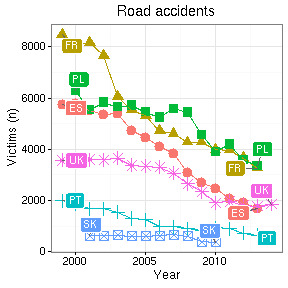
\includegraphics{2015-manu-roadacc-1}
\end{center}
\caption{Timeline indicating the number of people killed in road accidents in various countries based on Eurostat open data retrieved with the \CRANpkg{eurostat} package.}
\label{fig:transport}
\end{figure}




\section{Utilities}

Many entries in Table~\ref{tab:getdatatable} are not readily
interpretable, but a simple call \code{label\_eurostat(dat)} can be
used to convert the original identifier codes into human-readable
labels (Table~\ref{tab:getdatatable2}) based on translations
in the Eurostat database. Labels are available in English, France and
Germany.

The Eurostat database includes a variety of demographic and health
indicators. We see, for instance, that overweight varies remarkably
across different age groups (Figure~\ref{fig:bmi}A). Sometimes the
data sets require more complicated pre-processing. Let's consider, for
instance, the distribution of renewable energy sources in different
European countries. In order to summarise such data one needs to first
aggregate a multitude of possible energy sources into a smaller number
of coherent groups. Then one can use standard R tools to process the
data, chop country names, filter countries depending on production
levels, normalize the within country production. After a series of
transformations (see Appendix for the source code) we can finally plot
the data to discover that countries vary a lot in terms of renewable
energy sources (Figure~\ref{fig:bmi}B). Three-dimensional data sets
such as this can be conveniently visualized as triangular maps by
using the \CRANpkg{plotrix} \citep{plotrix} package.

The data sets are stored in cache by default to avoid repeated
downloads of identical data and to speed up the analysis. Storing
an exact copy of the retrieved raw data on the hard disk will also
support reproducibility when the source database is constantly
updated.



\begin{figure}
\setkeys{Gin}{width=0.5\textwidth}
\begin{center}
\begin{tabular}{cc}
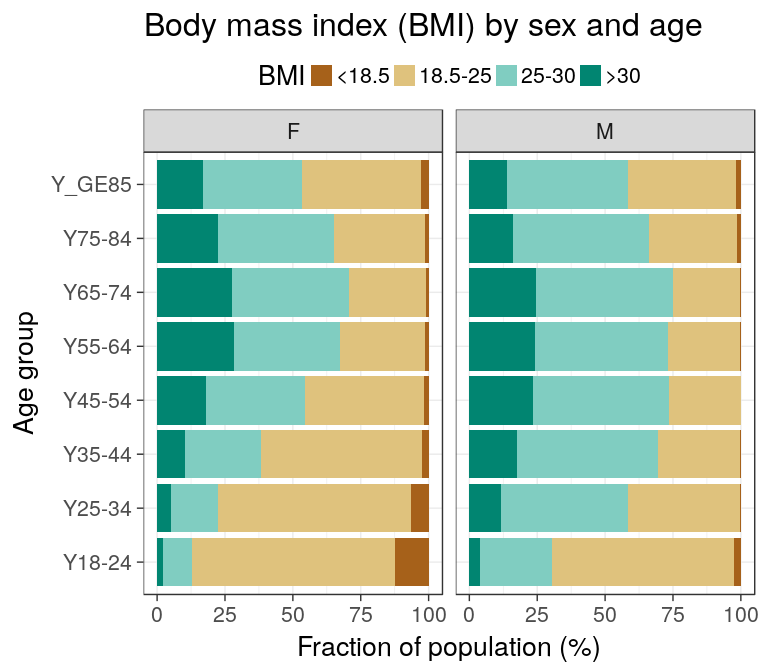
\includegraphics{2015-manu-bmi-1}
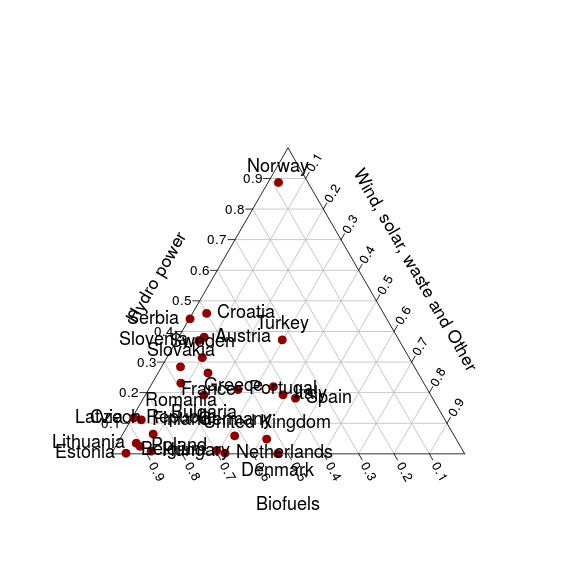
\includegraphics{2015-manu-energy-1}
\end{tabular}
\end{center}
\caption{{\bf A} The body-mass index (BMI) in different age groups in Poland (Eurostat table \texttt{hlth\_ehis\_de1}). {\bf B} Production of renewable energy in various countries in 2013 (Eurostat table \texttt{ten00081}). See the Appendix for the source code.}
\label{fig:bmi}
\end{figure}



\section{Geospatial information}

\subsection{Map visualizations}

The indicators in the Eurostat open data service are typically
available as annual time series grouped by country, and sometimes at
more refined temporal or geographic levels. Eurostat provides
complementary geospatial data on the corresponding administrative
statistical units to support visualizations at the appropriate
geographic resolution. The geospatial data sets are available as
standard
shapefiles\footnote{http://ec.europa.eu/eurostat/web/gisco/geodata/reference-data/administrative-units-statistical-units}. Let
us look at disposable income of private households (data identifier
tgs00026\footnote{http://ec.europa.eu/eurostat/en/web/products-datasets/-/TGS00026}). This
is provided at the geographic NUTS2 regions, the intermediate
territorial units in the Eurostat regional classifications, roughly
corresponding to provinces or states in each
country\footnote{http://ec.europa.eu/eurostat/web/nuts/overview}
(Figure~\ref{fig:mapexample}). The map is generated with:

\begin{example}
> # Loading required libraries
> library(eurostat)
> library(dplyr)
> library(ggplot2)

> # Downloading and manipulating the tabular data
> get_eurostat("tgs00026", time_format = "raw") %>% 
+   # subsetting to year 2005 and NUTS-3 level
+   dplyr::filter(time == 2005, nchar(as.character(geo)) == 4) %>%

+   # Classify the values the variable
+   dplyr::mutate(cat = cut_to_classes(values)) %>%

+   # Merge Eurostat data with geodata from Cisco
+   merge_eurostat_geodata(data=.,geocolumn="geo",resolution = "60", output_class ="df") %>%

+   # Plot map
+   ggplot(data=., aes(long,lat,group=group)) +
+   geom_polygon(aes(fill = cat),colour=alpha("white", 1/2),size=.2) +
+   scale_fill_manual(values=RColorBrewer::brewer.pal(n = 5, name = "Oranges")) +
+   labs(title="Dispostable household income") +
+   coord_map(project="orthographic", xlim=c(-22,34), ylim=c(35,70)) + theme_minimal() +
+   guides(fill = guide_legend(title = "EUR per Year",title.position = "top", title.hjust=0))
\end{example}


This demonstrates how the Eurostat statistics and geospatial data,
retrieved with the eurostat package, can be combined with the help of
additional visualization tools and other utilities including
\CRANpkg{grid} \citep{grid}, \CRANpkg{maptools} \citep{maptools}, \CRANpkg{rgdal} \citep{rgdal},
\CRANpkg{rgeos} \citep{rgeos}, \CRANpkg{scales} \citep{scales}, and
\CRANpkg{stringr} \citep{stringr}.

\begin{figure}
\setkeys{Gin}{width=0.7\textwidth}
\begin{center}
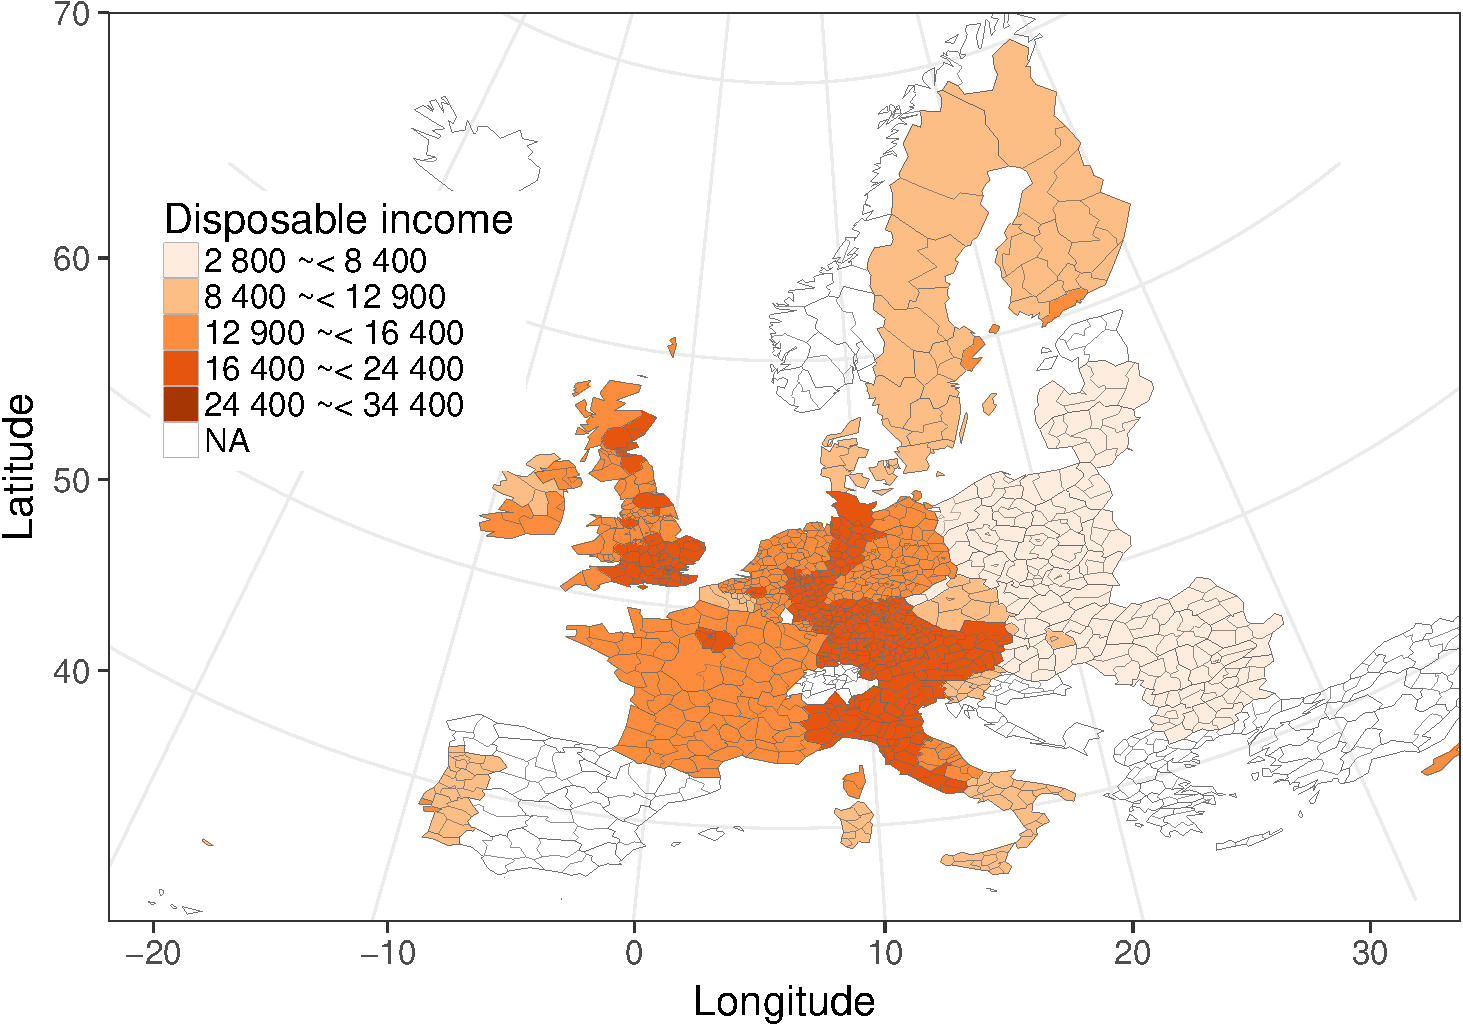
\includegraphics{2015-manu-mapexample-1}
\caption{Disposable income of private households across NUTS2-level national regions in European countries visualized based on geospatial data available from Eurostat.}
\label{fig:mapexample}
\end{center}
\end{figure}


\subsection{Default country groupings}

To facilitate the analysis and visualization of standard European
country groups, we have included ready-made country code lists. The
list of EFTA countries (Table~\ref{tab:efta}), for instance, is
retrieved with:

\begin{example}
> data(efta_countries)
\end{example}

\begin{table}[h]
\centering
\begin{tabular}{rll}
\toprule
  \hline
  & code & name \\ 
  \hline
  1 & IS & Iceland \\ 
  2 & LI & Liechtenstein \\ 
  3 & NO & Norway \\ 
  4 & CH & Switzerland \\ 
   \hline
\bottomrule   
\end{tabular}
\caption{The EFTA country listing from the eurostat R package.}
\label{tab:efta}
\end{table}

Similar lists are available for Euro area (ea\_countries), EU
(eu\_countries) and the EU candidate countries
(eu\_candidate\_countries). These auxiliary data sets facilitate
smooth selection of specific country groups for a closer analysis. The
full name and a two-letter identifier are provided for each country
according to the Eurostat database. The country codes follow the ISO
3166-1 alpha-2 standard, except that GB and GR are replaced by UK
(United Kingdom) and EL (Greece) in the Eurostat database,
respectively. Linking these country codes with external data sets can
be facilitated by conversions between different country coding
standards with the \CRANpkg{countrycode} package \citep{countrycode}.




\section{Summary}


By combining programmatic access to data with custom analysis and
visualization tools it is possible to facilitate a seamless automation
of the complete data analytical workflow from raw data to statistical
summaries and final publication. The \CRANpkg{eurostat} R package
provides convenient tools to access open data from Eurostat. It
exemplifies automated and transparent data retrieval from
institutional data repositories, featuring options such as search,
subsetting and cache. Moreover, it provides several functions to
facilitate the analysis and visualization of the Eurostat
data. Possible future extensions and improvements include
implementation of specific data representation formats that could be
used to harmonize the data representation with other related data
sources and to facilitate subsequent tool development. In particular,
we should take further advantage of the existing spatiotemporal data
structures that are available in R, such as those provided by
the \CRANpkg{spacetime} package \citep{spacetime}, and construct
wrapper functions to speed up routine operations such as the
visualization of the temporal and geospatial data sets. The source
code and installation instructions for the latest development version
of the eurostat package and this
manuscript\footnote{https://github.com/rOpenGov/eurostat} are
available via Github. The source code can be freely used, modified and
distributed under the BSD-2-clause (modified FreeBSD) license. Issues,
bug reports, pull requests, and other feedback are welcome.


\section*{Acknowledgements}

We are grateful to Eurostat for maintaining the open data service and
the rOpenGov\footnote{https://github.ropengov.io} for supporting R
package development. This work has been partially funded by Academy of
Finland (decision 293316). We also wish to thank all package
contributors.


\bibliography{lahti-huovari-kainu-biecek}

\address{Leo Lahti\\
  Department of Mathematics and Statistics\\
  PO Box 20014 University of Turku\\
  Finland\\}
\email{leo.lahti@iki.fi}

\address{Janne Huovari\\
  Pellervo Economic Research PTT\\
  Eerikinkatu 28 A 00180 Helsinki\\
  Finland\\}
\email{janne.huovari@ptt.fi}

\address{Markus Kainu\\
  Research Department, The Social Insurance Institution of Finland\\
  PO Box 450, 00101 Helsinki\\
  Finland\\}
\email{markus.kainu@kela.fi}

\address{Przemyslaw Biecek\\
  Faculty of Mathematics, Informatics, and Mechanics\\
  University of Warsaw\\
  Banacha 2, 02-097 Warsaw\\
  Poland\\}
\email{P.Biecek@mimuw.edu.pl}

\newpage

\section{Appendix}

Source code for the obesity example (Figure~\ref{fig:bmi}A):

\begin{example}
> library(dplyr)
> tmp1 <- get_eurostat("hlth_ehis_de1", time_format = "raw")
> tmp1 %>%
+  dplyr::filter( isced97 == "TOTAL" ,
+          sex != "T",
+          age != "TOTAL", geo == "PL") %>%
+  mutate(BMI = factor(bmi, 
+                      levels=c("LT18P5","18P5-25","25-30","GE30"), 
+                      labels=c("<18.5", "18.5-25", "25-30",">30"))) %>%
+  arrange(BMI) %>%
+  ggplot(aes(y=values, x=age, fill=BMI)) + geom_bar(stat="identity") +
+  facet_wrap(~sex) + coord_flip() +
+  theme(legend.position="top") +
+  ggtitle("Body mass index (BMI) by sex and age") +
+  xlab("% of population") + scale_fill_brewer(type = "div")
\end{example}


Source code for the renewable energy example (Figure~\ref{fig:bmi}B):

\begin{example}
# All sources of renewable energy are to be grouped into three sets
> dict <- c("Solid biofuels (excluding charcoal)" = "Biofuels",
+          "Biogasoline" = "Biofuels",
+          "Other liquid biofuels" = "Biofuels",
+          "Biodiesels" = "Biofuels",
+          "Biogas" = "Biofuels",
+          "Hydro power" = "Hydro power",
+          "Tide, Wave and Ocean" = "Hydro power",
+          "Solar thermal" = "Wind, solar, waste and Other",
+          "Geothermal Energy" = "Wind, solar, waste and Other",
+          "Solar photovoltaic" = "Wind, solar, waste and Other",
+          "Municipal waste (renewable)" = "Wind, solar, waste and Other",
+          "Wind power" = "Wind, solar, waste and Other",
+          "Bio jet kerosene" = "Wind, solar, waste and Other")
# Some cleaning of the data is required
> energy3 <- get_eurostat("ten00081") %>%
+  label_eurostat(dat) %>% 
+  filter(time == "2013-01-01",
+         product != "Renewable energies") %>%
+  mutate(nproduct = dict[as.character(product)], # just three categories
+         geo = gsub(geo, pattern=" \\(.*", replacement="")) %>%
+  select(nproduct, geo, values) %>% 
+  group_by(nproduct, geo) %>%
+  summarise(svalue = sum(values)) %>%
+  group_by(geo) %>%
+  mutate(tvalue = sum(svalue),
+         svalue = svalue/sum(svalue)) %>%
+  filter(tvalue > 1000,
+         !grepl(geo, pattern="^Euro")) %>% # only large countrie
+  spread(nproduct, svalue)
# Triangle plot
> library(plotrix)
> par(cex=0.75)
> plotrix::triax.plot(as.matrix(energy3[, c(3,5,4)]),
+                      show.grid = TRUE,
+                      label.points = TRUE, point.labels = energy3$geo,
+                      pch = 19)
\end{example}


